\documentclass{article}
\usepackage[utf8]{inputenc}
\setlength{\parskip}{5pt} % esp. entre parrafos
\setlength{\parindent}{0pt} % esp. al inicio de un parrafo
\usepackage{listings} % listings
\usepackage{color} %colores
\usepackage{amsmath} % mates
\usepackage[sort&compress,numbers]{natbib} % referencias
\usepackage{url} % que las URLs se vean lindos
\usepackage[top=15mm,left=20mm,right=20mm,bottom=25mm]{geometry} % margenes
\usepackage{hyperref} % ligas de URLs
\usepackage{graphicx} % poner figuras
\usepackage[spanish,es-tabla]{babel} % nombre tablas
\usepackage{caption}
\usepackage{subcaption}



\definecolor{mypink}{rgb}{0.976, 0.462, 0.847}
\definecolor{mygray}{rgb}{0.976, 0.980, 0.980}
\definecolor{myblue}{rgb}{0.258, 0.682, 1}
\definecolor{mypink2}{rgb}{0.525, 0.054, 0.4}
\lstset{ 
  backgroundcolor=\color{mygray},
  commentstyle=\color{myblue},
  keywordstyle=\color{mypink}, 
  numberstyle=\tiny\color{mypink}
  stringstyle=\color{mypink2}, 
  breaklines=true,
}

\title{Tarea 12}
\author{Eduardo Navarro}
\date{Noviembre 2021}

\begin{document}

\maketitle

\section{Introducción}

En esta práctica se analizó el Puntaje F \cite{fscore} para diversas probabilidades \texttt{"ne, g, b"} en un experimento factorial. Después se analizaron los resultados obtenidos.

\section{Desarrollo}
Con las instrucciones de la tarea \cite{redneuro} y lo visto en clase \cite{twitchsimu} se le hicieron modificaciones al código para obtener el Puntaje F \cite{fscore} a diversas probabilidades \texttt{"ne, g, b"}. Se añadieron cuatro \texttt{for} en total, tres para las probabilidades \texttt{"ne, g, b"} y otro \texttt{for} para las repeticiones. Se trabajó con las probabilidades en orden de la tabla \ref{tabla1}

\begin{table}[h!]
\centering
\caption{Probabilidades a estudiar.}
\label{tabla1}
\begin{tabular}{|c|r|r|r|}
\hline
\textbf{Combo} & \multicolumn{1}{c|}{\textbf{Negro}} & \multicolumn{1}{c|}{\textbf{Gris}} & \multicolumn{1}{c|}{\textbf{Blanco}} \\ \hline
n1g1b1 & 0.300 & 0.300 & 0.100 \\ \hline
n1g1b2 & 0.300 & 0.300 & 0.010 \\ \hline
n1g1b3 & 0.300 & 0.300 & 0.001 \\ \hline
n1g2b1 & 0.300 & 0.600 & 0.100 \\ \hline
n1g2b2 & 0.300 & 0.600 & 0.010 \\ \hline
n1g2b3 & 0.300 & 0.600 & 0.001 \\ \hline
n1g3b1 & 0.300 & 0.900 & 0.100 \\ \hline
n1g3b2 & 0.300 & 0.900 & 0.010 \\ \hline
n1g3b3 & 0.300 & 0.900 & 0.001 \\ \hline
n2g1b1 & 0.600 & 0.300 & 0.100 \\ \hline
n2g1b2 & 0.600 & 0.300 & 0.010 \\ \hline
n2g1b3 & 0.600 & 0.300 & 0.001 \\ \hline
n2g2b1 & 0.600 & 0.600 & 0.100 \\ \hline
n2g2b2 & 0.600 & 0.600 & 0.010 \\ \hline
n2g2b3 & 0.600 & 0.600 & 0.001 \\ \hline
n2g3b1 & 0.600 & 0.900 & 0.100 \\ \hline
n2g3b2 & 0.600 & 0.900 & 0.010 \\ \hline
n2g3b3 & 0.600 & 0.900 & 0.001 \\ \hline
n3g1b1 & 0.990 & 0.300 & 0.100 \\ \hline
n3g1b2 & 0.990 & 0.300 & 0.010 \\ \hline
n3g1b3 & 0.990 & 0.300 & 0.001 \\ \hline
n3g2b1 & 0.990 & 0.600 & 0.100 \\ \hline
n3g2b2 & 0.990 & 0.600 & 0.010 \\ \hline
n3g2b3 & 0.990 & 0.600 & 0.001 \\ \hline
n3g3b1 & 0.990 & 0.900 & 0.100 \\ \hline
n3g3b2 & 0.990 & 0.900 & 0.010 \\ \hline
n3g3b3 & 0.990 & 0.900 & 0.001 \\ \hline
\end{tabular}
\end{table}

\begin{lstlisting} [language=R, caption= Código para la obtención del Puntaje F para diversas probabilidades.] 
neg<-c(0.3,0.6,0.99)
gri<-c(0.3,0.6,0.9)
bla<-c(0.1,0.01,0.001)
datos=data.frame()

j<-15

for(ne in neg){
for(g in gri){
for(b in bla){
  
for(rep in 1:j){
    


modelos <- read.csv("digits.txt", sep=" ", header=FALSE, stringsAsFactors=F)
modelos[modelos=='n'] <- ne
modelos[modelos=='g'] <- g
modelos[modelos=='b'] <- b
...
print(contadores)

precision <- diag(contadores) / colSums(contadores[,1:10])
recall <- diag(contadores) / rowSums(contadores)
fscore <- (2 * precision * recall) / (precision + recall) 
datos=rbind(datos,c(rep,ne,g,b,fscore))

}
}
}
}

names(datos) <- c("Replica", "Negro","Gris","Blanco","0", "1","2","3","4","5","6","7","8","9")
\end{lstlisting}

Con esto se generaron los datos de la tabla \ref{tabla2}

\begin{table}[h!]
\centering
\caption{Ejemplo de datos obtenidos.}
\label{tabla2}
\scalebox{0.9}{
\begin{tabular}{|c|r|r|r|r|r|r|r|r|r|r|r|r|r|}
\hline
\textbf{Réplica} & \multicolumn{1}{c|}{\textbf{Negro}} & \multicolumn{1}{c|}{\textbf{Gris}} & \multicolumn{1}{c|}{\textbf{Blanco}} & \multicolumn{1}{c|}{\textbf{0}} & \multicolumn{1}{c|}{\textbf{1}} & \multicolumn{1}{c|}{\textbf{2}} & \multicolumn{1}{c|}{\textbf{3}} & \multicolumn{1}{c|}{\textbf{4}} & \multicolumn{1}{c|}{\textbf{5}} & \multicolumn{1}{c|}{\textbf{6}} & \multicolumn{1}{c|}{\textbf{7}} & \multicolumn{1}{c|}{\textbf{8}} & \multicolumn{1}{c|}{\textbf{9}} \\ \hline
1 & 0.3000 & 0.3000 & 0.1000 & 0.0513 & 0.1013 & 0.0588 & 0.1569 & 0.0645 & 0.0870 & 0.1111 & 0.0417 &  & 0.1176 \\ \hline
2 & 0.3000 & 0.3000 & 0.1000 & 0.1667 & 0.0741 & 0.1356 & 0.1200 & 0.1960 & 0.0727 & 0.0444 & 0.0937 & 0.1025 &  \\ \hline
3 & 0.3000 & 0.3000 & 0.1000 & 0.0823 & 0.1176 & 0.0465 & 0.0741 &  & 0.0857 &  & 0.0740 &  &  \\ \hline
4 & 0.3000 & 0.3000 & 0.1000 & 0.1778 & 0.1579 & 0.0755 & 0.0444 & 0.1290 & 0.0526 & 0.0769 & 0.1429 & 0.0378 &  \\ \hline
\end{tabular}}
\end{table}

A los datos de la tabla \ref{tabla2} se le agregó otra columna para posteriormente reordenarla en la tabla \ref{tabla3}.

\begin{lstlisting} [language=R, caption= Código para la adición de la columna. El reordenamiento de datos y la gráfica.]
library(ggplot2)
library(tidyr)

etiquetas=rep(c("n1g1b1","n1g1b2","n1g1b3","n1g2b1","n1g2b2","n1g2b3","n1g3b1","n1g3b2","n1g3b3",
              "n2g1b1","n2g1b2","n2g1b3","n2g2b1","n2g2b2","n2g2b3","n2g3b1","n2g3b2","n2g3b3",
              "n3g1b1","n3g1b2","n3g1b3","n3g2b1","n3g2b2","n3g2b3","n3g3b1","n3g3b2","n3g3b3"),
            times=c(j,j,j,j,j,j,j,j,j,j,j,j,j,j,j,j,j,j,j,j,j,j,j,j,j,j,j))

datos$combo <- etiquetas 

library(reshape2)
dat.m <- melt(datos,id.vars='combo', measure.vars=c('0','1','2','3','4','5','6','7','8','9'))
library(ggplot2)

ggplot(dat.m, aes(x= combo, y= value, fill= combo)) + # fill=name allow to automatically dedicate a color for each group
  geom_boxplot()+ labs(x="Combo", y= "Puntaje F") +
  theme(axis.text.x = element_text(angle = 90, vjust = 0.5, hjust=1))+
  geom_violin(fill="green", color="yellow",alpha = 5/10)
\end{lstlisting}

\begin{table}[h!]
\centering
\caption{Ejemplo de datos reordenados obtenidos.}
\label{tabla3}
\begin{tabular}{|c|r|r|}
\hline
\textbf{combo} & \multicolumn{1}{c|}{\textbf{variable}} & \multicolumn{1}{c|}{\textbf{value}} \\ \hline
n1g1b1 & 0 & 0.0513 \\ \hline
n1g1b1 & 0 & 0.1667 \\ \hline
n1g1b1 & 0 & 0.0822 \\ \hline
n1g1b1 & 0 & 0.1778 \\ \hline
\end{tabular}
\end{table}

Con los datos de la tabla \ref{tabla3} se hizo la gráfica \ref{grafica1}

\begin{figure} [h!]% figura
\renewcommand{\figurename}{Gráfica}
    \centering
    \caption{ Puntaje F a diversas probabilidades.}
    \label{grafica1}
    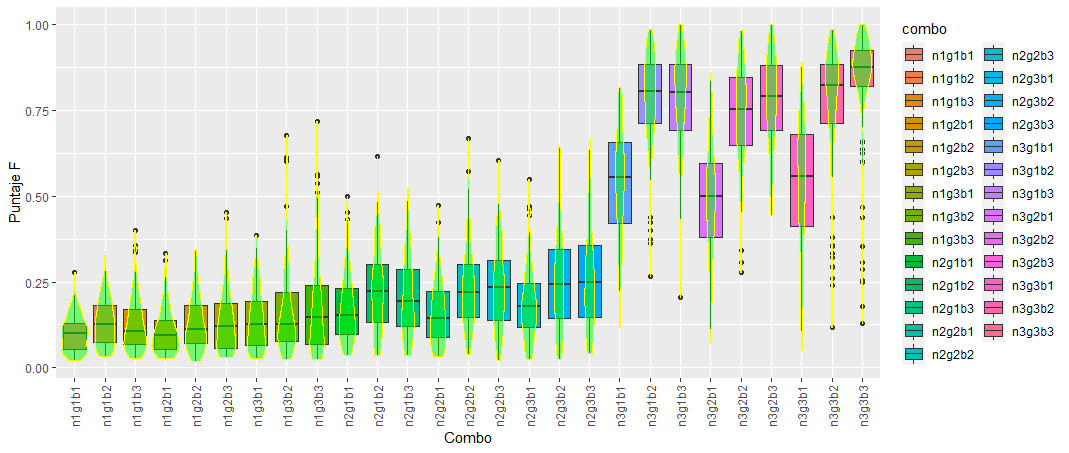
\includegraphics[width=175mm]{grafica1.png} % archivo
\end{figure}

Se realizaron pruebas estadísticas de  Shapiro–Wilk \cite{shapiro} y Kruskal-Wallis \cite{Kruskall}.

\begin{lstlisting} [language=R, caption= Código para la obtención de los datos estadísticos.]

library(tidyverse)

valorf<-dat.m%>%
  group_by(combo) %>%
  summarise(
    
    promedio = mean(value, na.rm = TRUE),
    desviacion_std = sd(value, na.rm = TRUE),
    varianza = sd(value, na.rm = TRUE)^2,
    mediana = median(value, na.rm = TRUE),
    rango_intercuartil = IQR(value, na.rm = TRUE)
  )

fshapiro<-tapply(dat.m$value, dat.m$combo, shapiro.test)

kruskal.test(value~combo, data=dat.m)
\end{lstlisting}

\begin{table}[h!]
\centering
\caption{Datos estadísticos obtenidos.}
\label{tabla4}
\begin{tabular}{|c|r|r|r|r|r|}
\hline
\textbf{Combo} & \multicolumn{1}{c|}{\textbf{Promedio}} & \multicolumn{1}{c|}{\textbf{Desviacion std}} & \multicolumn{1}{c|}{\textbf{Varianza}} & \multicolumn{1}{c|}{\textbf{Mediana}} & \multicolumn{1}{c|}{\textbf{Rango intercuartil}} \\ \hline
n1g1b1 & 0.1007 & 0.0496 & 0.0025 & 0.1013 & 0.0743 \\ \hline
n1g1b2 & 0.1316 & 0.0654 & 0.0043 & 0.1250 & 0.1068 \\ \hline
n1g1b3 & 0.1280 & 0.0761 & 0.0058 & 0.1071 & 0.0997 \\ \hline
n1g2b1 & 0.1088 & 0.0637 & 0.0041 & 0.0934 & 0.0843 \\ \hline
n1g2b2 & 0.1305 & 0.0760 & 0.0058 & 0.1111 & 0.1103 \\ \hline
n1g2b3 & 0.1355 & 0.0872 & 0.0076 & 0.1206 & 0.1298 \\ \hline
n1g3b1 & 0.1399 & 0.0849 & 0.0072 & 0.1263 & 0.1265 \\ \hline
n1g3b2 & 0.1688 & 0.1294 & 0.0167 & 0.1269 & 0.1418 \\ \hline
n1g3b3 & 0.1822 & 0.1426 & 0.0203 & 0.1461 & 0.1721 \\ \hline
n2g1b1 & 0.1724 & 0.0966 & 0.0093 & 0.1538 & 0.1339 \\ \hline
n2g1b2 & 0.2283 & 0.1209 & 0.0146 & 0.2222 & 0.1710 \\ \hline
n2g1b3 & 0.2110 & 0.1192 & 0.0142 & 0.1920 & 0.1643 \\ \hline
n2g2b1 & 0.1605 & 0.0923 & 0.0085 & 0.1451 & 0.1335 \\ \hline
n2g2b2 & 0.2365 & 0.1210 & 0.0146 & 0.2208 & 0.1544 \\ \hline
n2g2b3 & 0.2360 & 0.1217 & 0.0148 & 0.2352 & 0.1760 \\ \hline
n2g3b1 & 0.1903 & 0.1070 & 0.0114 & 0.1777 & 0.1275 \\ \hline
n2g3b2 & 0.2586 & 0.1492 & 0.0222 & 0.2424 & 0.2016 \\ \hline
n2g3b3 & 0.2667 & 0.1534 & 0.0235 & 0.2471 & 0.2108 \\ \hline
n3g1b1 & 0.5387 & 0.1641 & 0.0269 & 0.5529 & 0.2345 \\ \hline
n3g1b2 & 0.7772 & 0.1386 & 0.0192 & 0.8027 & 0.1737 \\ \hline
n3g1b3 & 0.7782 & 0.1412 & 0.0199 & 0.8000 & 0.1932 \\ \hline
n3g2b1 & 0.4871 & 0.1774 & 0.0314 & 0.5000 & 0.2153 \\ \hline
n3g2b2 & 0.7382 & 0.1426 & 0.0203 & 0.7520 & 0.1980 \\ \hline
n3g2b3 & 0.7715 & 0.1345 & 0.0180 & 0.7908 & 0.1900 \\ \hline
n3g3b1 & 0.5285 & 0.1903 & 0.0362 & 0.5569 & 0.2662 \\ \hline
n3g3b2 & 0.7685 & 0.1763 & 0.0310 & 0.8214 & 0.1721 \\ \hline
n3g3b3 & 0.8343 & 0.1622 & 0.0263 & 0.8727 & 0.1021 \\ \hline
\end{tabular}
\end{table}

\newpage

\begin{table}[h!]
\centering
\caption{Resultados de la prueba Shapiro–Wilk.}
\label{tabla5}
\begin{tabular}{|c|r|r|}
\hline
Combo & \multicolumn{1}{c|}{W} & \multicolumn{1}{c|}{P} \\ \hline
n1g1b1 & 0.9552 & 0.0005 \\ \hline
n1g1b2 & 0.9607 & 0.0017 \\ \hline
n1g1b3 & 0.9097 & $4.89\times 10^{-7}$  \\ \hline
n1g2b1 & 0.9011 & $1.85\times 10^{-7}$  \\ \hline
n1g2b2 & 0.9316 & $1.54\times 10^{-5}$ \\ \hline
n1g2b3 & 0.9071 & $3.21\times 10^{-7}$ \\ \hline
n1g3b1 & 0.9322 & $1.81\times 10^{-5}$ \\ \hline
n1g3b2 & 0.8300 & $1.06\times 10^{-10}$ \\ \hline
n1g3b3 & 0.8678 & $3.22\times 10^{-9}$ \\ \hline
n2g1b1 & 0.9397 & $9.24\times 10^{-6}$ \\ \hline
n2g1b2 & 0.9684 & 0.0022 \\ \hline
n2g1b3 & 0.9535 & $8.31\times 10^{-5}$ \\ \hline
n2g2b1 & 0.9430 & $2.61\times 10^{-5}$ \\ \hline
n2g2b2 & 0.9684 & 0.0002 \\ \hline
n2g2b3 & 0.9718 & 0.0063 \\ \hline
n2g3b1 & 0.9467 & $6.07\times 10^{-5}$ \\ \hline
n2g3b2 & 0.9582 & 0.0002 \\ \hline
n2g3b3 & 0.9513 & $9.34\times 10^{-5}$ \\ \hline
n3g1b1 & 0.9787 & 0.02014 \\ \hline
n3g1b2 & 0.9278 & $7.00\times 10^{-7}$ \\ \hline
n3g1b3 & 0.9398 & $5.15\times 10^{-6}$ \\ \hline
n3g2b1 & 0.9871 & 0.1856 \\ \hline
n3g2b2 & 0.9682 & 0.0015 \\ \hline
n3g2b3 & 0.9647 & 0.0006 \\ \hline
n3g3b1 & 0.9700 & 0.0024 \\ \hline
n3g3b2 & 0.8406 & $1.80\times 10^{-11}$ \\ \hline
n3g3b3 & 0.7192 & $1.35\times 10^{-15}$ \\ \hline
\end{tabular}
\end{table}

\begin{table}[h!]
\centering
\caption{Resultados de la prueba Kruskal-Wallis.}
\label{tabla6}
\begin{tabular}{|c|c|}
\hline
\textbf{H(26)} & \textbf{P} \\ \hline
\multicolumn{1}{|r|}{2590.2} & \multicolumn{1}{r|}{$2.20\times 10^{-16}$} \\ \hline
\end{tabular}
\end{table}

Para el reto 1 se modificó el documento para que leyera 12 símbolos ASCII aparte de los números y se obtubo la figura \ref{grafica2}, de igual forma se obtubo una matriz.
\newpage

\begin{figure} [h!]% figura
    \centering
    \caption{ Números y símbolos ASCII obtenidos.}
    \label{grafica2}
    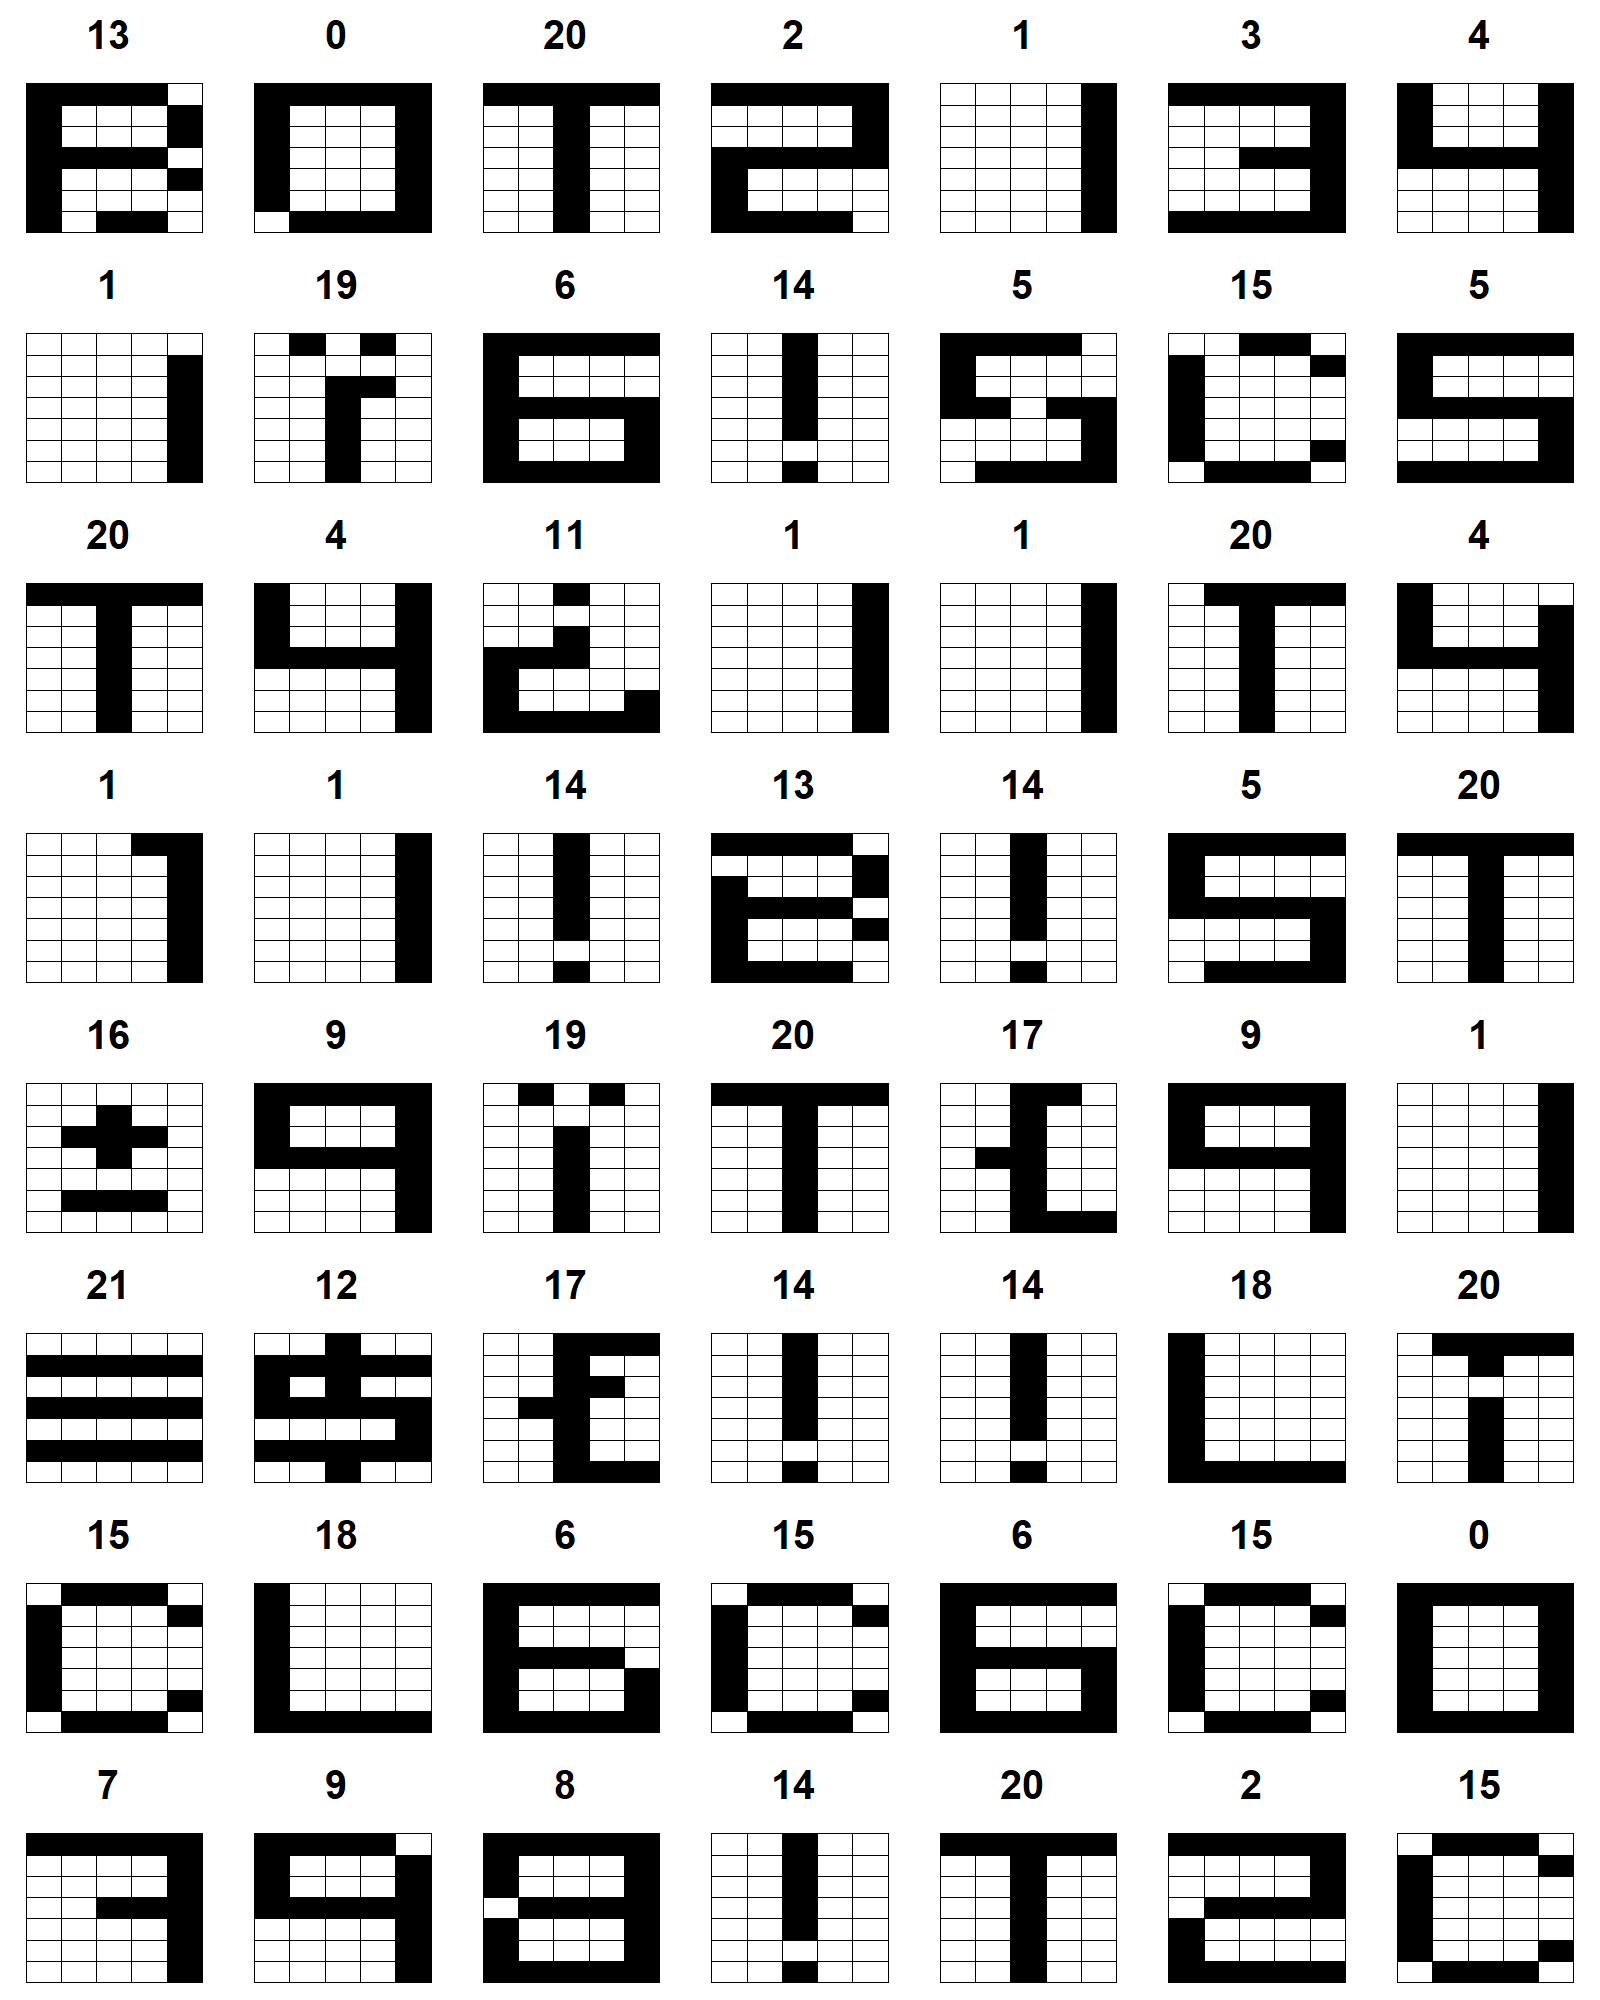
\includegraphics[width=150mm]{p12g.png} % archivo
\end{figure}

\begin{lstlisting} [language=R, caption= Código para el reto 1.]

modelos <- read.csv("digitosr1.txt", sep=" ", header=FALSE, stringsAsFactors=F)
modelos[modelos=='n'] <- 0.995
modelos[modelos=='g'] <- 0.92
modelos[modelos=='b'] <- 0.002

r <- 7
c <- 5
dim <- r * c

tasa <- 0.15
tranqui <- 0.99

tope <- 21
digitos <- 0:tope
\end{lstlisting}

\begin{lstlisting} [language=R, caption= Matriz obtenida.]
    0  1  2  3 4  5 6 7  8 9 10 11 12 13 14 15 16 17 18 19 20 21 <NA>
0   0  0  0  0 0  0 0 0  1 0 11  0  0  0  1  1  0  0  0  0  0  0    0
1   0  8  0  0 0  0 0 0  0 0  0  0  0  0  0  0  0  0  0  0  0  0    0
2   0  0 12  2 0  0 0 0  0 0  0  0  0  0  0  0  0  0  0  0  0  0    0
3   0  0  0 12 0  0 0 1  0 0  0  3  0  0  0  0  0  0  0  0  0  0    0
4  15  0  0  0 0  0 0 0  0 0  0  0  0  0  0  0  0  0  0  0  0  0    0
5   0 14  0  0 0  3 0 0  0 1  0  0  0  1  0  0  0  0  0  0  0  0    0
6   0  0  0  0 9  2 0 0  0 0  0  0  0  0  0  0  0  0  0  0  0  0    0
7   0  0  0  0 0 13 0 1  0 1  0  0  0  0  0  0  0  0  0  0  0  0    0
8   0  1  0  0 0  0 0 0 10 0  0  3  0  0  2  0  0  0  0  0  0  0    0
9   0  0  0  0 8  0 0 0  0 0  0  0  1  0  0  0  0  0  0  0  0  0    0
10  0  0  0  0 0  0 0 0  0 0  6  0  0  0  2  1  0  0  0  0  0  0    0
11  0  1  1 15 0  0 0 0  0 1  4  2  0  0  0  1  0  0  0  0  0  0    0
12  0  0  0  0 0  0 0 0  0 0  0  0 11  1  0  0  0  0  0  0  0  0    3
13  0  0  0  0 0  0 0 0  0 0  0  0  0  0  2 17  0  0  0  0  0  0    0
14  0  0  0  0 0  0 0 0  0 0  0  0 12  0  0  0  0  0  0  0  0  0    1
15  0  0  0  0 0  0 0 0  0 0  0  1  0  0  2 11  0  0  0  0  0  0    0
16  0  0  0  0 0  0 0 0  0 0  0  0  0  0  0  0  0  0  0  1  0  0   12
17  0  2  0  0 0  0 0 0  0 0  0  0  0  0  0  0  0 11  0  0  0  0    0
18  0  0  0  0 0  0 0 0  0 0  0  0  0  0  0  0  0  0  9  0  0  0    0
19  0  0  0  0 0  0 0 0  0 0  0  0  0  0  0  0  0  0  5  0  0  0    3
20  0  0  0  0 0  0 0 0  0 0  0  0  0  0  0  0  9  0  0  0  0  0    0
21  0  0  0  0 0  0 0 0  0 0  0  0  0  2  0  0  0  0  0  0  0 12    2
\end{lstlisting}



\section{Conclusiones}
De la gráfica se puede concluir que las variables de las probabilidadaes tienen influencia en distinta medida correlacionada entre ellas. Se puede observar que la probabilidad en negro tiene una gran influencia en valores altos cercanos a 1 y del valor blanco se tiene influencia en valores cercanos a 0, el valor de gris muestra un ligero aumento al puntaje f entre grupos aumentando la concentración de valores altos conforme aumenta en conjunto con los otros valores mientras el blanco disminuya. Del reto se consiguió generar los doce símbolos ASCII.

\bibliography{referencias}
\bibliographystyle{plainnat}
\end{document}
